\chapter{Introducción}
\label{capitulo1}
%Históricamente, se ha visto un aumento en la sofisticación, velocidad, impacto y 
cantidad de los ataques informáticos. Por ello es necesario que las estrategias 
de defensa se adapten a los nuevos actores y ataques. Para responder a esto, las 
organizaciones han tenido que recurrir al intercambio de información de amenazas 
con el fin de tener un mejor panorama de las actividades de sus adversarios 
y así ayudar a administrar sus recursos de forma de obtener el mejor resultado 
posible de sus defensas. \\

Las aproximaciones tradicionales de seguridad tienen como objetivo entender y 
registrar vulnerabilidades, debilidades y configuraciones necesarias pero 
insuficientes. Para defenderse, las organizaciones tienen estrategias basadas en 
alertas que buscan bloquear los ataques y arreglar las vulnerabilidades. Si bien dichas estrategias pueden ser efectivas contra algunas 
amenazas no logran detener ataques avanzados o proveer información sobre las 
actividades de un atacante luego de que ingresó a la red. Una estrategia más 
adecuada es basarse en \textbf{\textit{cyber kill-chain}}, en esta estrategia se busca 
descomponer las fases de un ataque con la finalidad de obtener una mejor 
comprensión del ataque y el atacante, así como mejorar las posibilidades de 
defensa.

\begin{figure}[H]
  \label{fig:kill_chain}
  \centering
  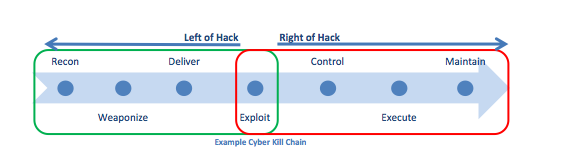
\includegraphics[scale=0.55]{./images/killChain.png}
    \caption{Cyber kill-chain \protect\cite{b1}}
\end{figure}

Como se ve en la figura~\ref{fig:kill_chain}, los primeros pasos de esta estrategia representan una 
oportunidad para detectar y mitigar las amenazas de forma proactiva antes de que 
al adversario realice un acceso no autorizado en los sistemas de la 
organización. En los pasos posteriores es donde se realiza la detección, 
respuesta y aseguramiento de los activos más importantes. Al entender al 
adversario, se puede tener una mejor oportunidad para descubrir sus intenciones 
y responder al ataque. Entender la amenaza permite la toma de mejores 
decisiones, dando prioridad a los recursos y así tener una ventaja ante el atacante. 
El resultado de defensas en base a inteligencia es una mejor opción que las 
respuestas a los ataques dado que estos ajustan sus operaciones basándose en el 
éxito o falla de sus intentos. En un modelo como el de la figura~\ref{fig:kill_chain} los intentos 
del adversario pueden ser reconocidos, logrando que los defensores tengan la 
posibilidad de ajustar sus tácticas para que al adversario le sea más 
difícil alcanzar sus objetivos.\\

Compartir información con socios y comunidades de confianza le permite a las 
organizaciones tener un conjunto de datos relevante para lograr una 
identificación precisa de la amenaza. Por medio de este intercambio, cada organización 
puede entender mejor las amenazas, no 
solo de forma abstracta sino que también con evidencias específicas que 
indiquen la presencia del atacante. Las tareas de cyber inteligencia permiten 
anticipar y mitigar las amenazas antes de que sean difíciles de encontrar y 
erradicar utilizando los métodos tradicionales de detección y respuesta. Con la 
información recolectada los analistas pueden agrupar patrones de actividades 
similares, atribuir actividades a ciertos actores, identificar e implementar 
estrategias para mitigar ataques de forma rápida y anticiparse al lanzamiento de 
ataques similares en el futuro. Para aprovechar de forma adecuada los beneficios 
de la cyber inteligencia, las organizaciones deben compartir la información 
recolectada con socios de su confianza.\\

Por medio del análisis del comportamiento de los adversarios en distintos 
objetivos y en un período de tiempo adecuado, los defensores son capaces de 
identificar un conjunto importante de indicadores, tácticas, técnicas y 
procedimientos. De esta forma se obtiene información de los objetivos y las 
estrategias lo cual permite al defensor predecir el comportamiento del atacante y 
generar defensas dinámicas. Dada la forma y complejidad con la cual evolucionan 
las amenazas, la velocidad con la cual ocurren los eventos y la basta cantidad 
de datos que se deberían intercambiar, es necesario establecer una forma 
automática para ayudar a los analistas y tomadores de decisión a llevar a cabo 
acciones defensivas.\\

Existen múltiples métodos para el intercambio de información y estos juegan un rol 
importante en los tipos, volúmenes y naturaleza de la información compartida 
con la comunidad. Algunos de estos medios de intercambio limitan el tipo de 
contenido que es compartido mientras que otros promueven ciertos tipos de 
intercambio. Los procesos para compartir información son manuales, llevan mucho 
tiempo, son repetitivos y en muchos casos requieren que las organizaciones 
reescriban o traduzcan la información a una amplia variedad de formatos. Otro 
problema que se presenta cuando se quiere intercambiar información es la 
utilización de tecnologías y/o formatos propietarios, esto provoca la necesidad 
de desarrollar scripts y módulos para permitir compartir información por fuera 
de las comunidades. Para aquellas comunidades con algún grado de automatización, 
sus modelos son generalmente bajos en prestaciones y usan soluciones 
propietarias, comerciales o adaptadas a su comunidad.\\

La mayoría de dichos 
métodos no permiten el consumo de información de amenazas de forma automática, 
esto hace que rutinariamente las organizaciones deban tomar dicha información y 
sintetizarla en sus bases de datos locales. Si bien los métodos utilizados en la 
actualidad han ayudado a mejorar las capacidades defensivas de numerosas 
organizaciones, éstas no han logrado explotar su máximo potencial.\\

La automatización requiere de información de calidad, esto 
no puede ser logrado adecuadamente con los distintos productos y sistemas de hoy en 
día. Para lograr un nivel adecuado de automatización es necesario contar con un 
estándar el cual tenga representaciones estructuradas de información, de ésta 
forma se puede lograr un mejor aprovechamiento de los datos sin saber de 
antemano quien los provee. Dicha información debe ser legible por un humano y 
parseable por una máquina. Estos requerimientos tienen varias justificaciones, 
primero que nada, un analista podría realizar un análisis que es inapropiado 
para ser automatizado o que sea focalizado en tomas de decisiones por parte de 
personas. También podría ser de interés que un analista tenga conocimiento de la 
situación actual,  de la fidelidad de las fuentes o de los métodos utilizados 
para producir la información. Por lo dicho anteriormente, es necesario la 
existencia de un estándar con una representación estructurada de la información, siendo ésta 
expresiva, flexible, extensible, automatizable y legible. Además se deben contar 
con medios para permitir el intercambio seguro y confiable de información entre 
distintas organizaciones.\\

Si bien existen varios esfuerzos para crear herramientas con las características 
presentadas, la realidad es que ninguno de ellos ha logrado su cometido. El 
objetivo de dicha herramienta debería ser:
\begin{itemize}
  \item Permitir compartir información de forma más rápida y precisa.
  \item Reducir el análisis humano y liberar a los recursos humanos para 
  realizar trabajo de análisis más valioso.
  \item Permitir que las amenazas más conocidas sean analizadas por 
  computadoras.
  \item Permitir que se comparta de forma automática un gran número de datos, 
  siendo estos datos complejos. Esto debería permitir una defensa activa.
  \item Proteger la información intercambiada.
  \item Permitir que se agregue información a las bases locales con discreción y 
  limitando el número de analistas que acceden a la información. Dicha 
  información debe tener datos de contexto.
  \item Permitir la colaboración de analistas de distintas organizaciones en los 
  incidentes.
\end{itemize}


\section{Contexto}
\label{capitulo1:contexto}
Este proyecto se desarrolla en el contexto de los temas de investigación y trabajo desarrollados en el Instituto de Computación, en particular dentro del grupo de seguridad informática (GSI) y del equipo de Respuesta a incidentes de Tilsor S.A (CSIRT Tilsor). Se interaccionará y coordinará eventualmente con otras personas y/o organizaciones que estén trabajando en temas afines.

\section{Motivación}
\label{capitulo1:motivacion}
Históricamente, se ha visto un aumento en la sofisticación, velocidad, impacto y 
cantidad de los ataques informáticos. Por ello es necesario que las estrategias 
de defensa se adapten a los nuevos actores y ataques. Para responder a esto, las 
organizaciones han tenido que recurrir al intercambio de información de amenazas 
con el fin de tener un mejor panorama de las actividades de sus adversarios 
y así ayudar a administrar sus recursos de forma de obtener el mejor resultado 
posible de sus defensas. \\

Las aproximaciones tradicionales de seguridad tienen como objetivo entender y 
registrar vulnerabilidades, debilidades y configuraciones necesarias pero 
insuficientes. Para defenderse, las organizaciones tienen estrategias basadas en 
alertas que buscan bloquear los ataques y arreglar las vulnerabilidades. Si bien dichas estrategias pueden ser efectivas contra algunas 
amenazas no logran detener ataques avanzados o proveer información sobre las 
actividades de un atacante luego de que ingresó a la red. Una estrategia más 
adecuada es basarse en \textbf{\textit{cyber kill-chain}}, en esta estrategia se busca 
descomponer las fases de un ataque con la finalidad de obtener una mejor 
comprensión del ataque y el atacante, así como mejorar las posibilidades de 
defensa.

\begin{figure}[H]
  \centering
  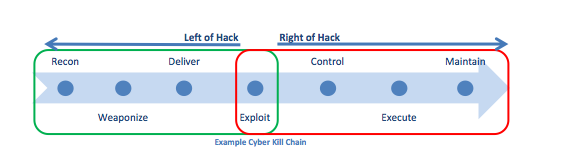
\includegraphics[scale=0.55]{./images/killChain.png}
    \caption{Cyber kill-chain \protect\cite{b1}}
      \label{fig:kill_chain}
\end{figure}

Como se ve en la figura~\ref{fig:kill_chain}, los primeros pasos de esta estrategia representan una 
oportunidad para detectar y mitigar las amenazas de forma proactiva antes de que 
al adversario realice un acceso no autorizado en los sistemas de la 
organización. En los pasos posteriores es donde se realiza la detección, 
respuesta y aseguramiento de los activos más importantes. Al entender al 
adversario, se puede tener una mejor oportunidad para descubrir sus intenciones 
y responder al ataque. Entender la amenaza permite la toma de mejores 
decisiones, dando prioridad a los recursos y así tener una ventaja ante el atacante. 
El resultado de defensas en base a inteligencia es una mejor opción que las 
respuestas a los ataques dado que estos ajustan sus operaciones basándose en el 
éxito o falla de sus intentos. En un modelo como el de la figura~\ref{fig:kill_chain} los intentos 
del adversario pueden ser reconocidos, logrando que los defensores tengan la 
posibilidad de ajustar sus tácticas para que al adversario le sea más 
difícil alcanzar sus objetivos.\\

Compartir información con socios y comunidades de confianza le permite a las 
organizaciones tener un conjunto de datos relevante para lograr una 
identificación precisa de la amenaza. Por medio de este intercambio, cada organización 
puede entender mejor las amenazas, no 
solo de forma abstracta sino que también con evidencias específicas que 
indiquen la presencia del atacante. Las tareas de cyber inteligencia permiten 
anticipar y mitigar las amenazas antes de que sean difíciles de encontrar y 
erradicar utilizando los métodos tradicionales de detección y respuesta. Con la 
información recolectada los analistas pueden agrupar patrones de actividades 
similares, atribuir actividades a ciertos actores, identificar e implementar 
estrategias para mitigar ataques de forma rápida y anticiparse al lanzamiento de 
ataques similares en el futuro. Para aprovechar de forma adecuada los beneficios 
de la cyber inteligencia, las organizaciones deben compartir la información 
recolectada con socios de su confianza.\\

Por medio del análisis del comportamiento de los adversarios en distintos 
objetivos y en un período de tiempo adecuado, los defensores son capaces de 
identificar un conjunto importante de indicadores, tácticas, técnicas y 
procedimientos. De esta forma se obtiene información de los objetivos y las 
estrategias lo cual permite al defensor predecir el comportamiento del ataque y 
generar defensas dinámicas. Dada la forma y complejidad con la cual evolucionan 
las amenazas, la velocidad con la cual ocurren los eventos y la basta cantidad 
de datos que se deberían intercambiar, es necesario establecer una forma 
automática para ayudar a los analistas y tomadores de decisión a llevar a cabo 
acciones defensivas.\\

Existen múltiples métodos para el intercambio de información y estos juegan un rol 
importante en los tipos, volúmenes y naturaleza de la información compartida 
con la comunidad. Algunos de estos medios de intercambio limitan el tipo de 
contenido que es compartido mientras que otros promueven ciertos tipos de 
intercambio. Los procesos para compartir información son manuales, llevan mucho 
tiempo, son repetitivos y en muchos casos requieren que las organizaciones 
reescriban o traduzcan la información a una amplia variedad de formatos. Otro 
problema que se presenta cuando se quiere intercambiar información es la 
utilización de tecnologías y/o formatos propietarios, esto provoca la necesidad 
de desarrollar scripts y módulos para permitir compartir información por fuera 
de las comunidades. Para aquellas comunidades con algún grado de automatización, 
sus modelos son generalmente bajos en prestaciones y usan soluciones 
propietarias, comerciales o adaptadas a su comunidad.\\

La mayoría de dichos 
métodos no permiten el consumo de información de amenazas de forma automática, 
esto hace que rutinariamente las organizaciones deban tomar dicha información y 
sintetizarla en sus bases de datos locales. Si bien los métodos utilizados en la 
actualidad han ayudado a mejorar las capacidades defensivas de numerosas 
organizaciones, éstas no han logrado explotar su máximo potencial.\\

La automatización requiere de información de calidad, esto 
no puede ser logrado adecuadamente con los distintos productos y sistemas de hoy en 
día. Para lograr un nivel adecuado de automatización es necesario contar con un 
estándar el cual tenga representaciones estructuradas de información, de ésta 
forma se puede lograr un mejor aprovechamiento de los datos sin saber de 
antemano quien los provee. Dicha información debe ser legible por un humano y 
parseable por una máquina. Estos requerimientos tienen varias justificaciones, 
primero que nada, un analista podría realizar un análisis que es inapropiado 
para ser automatizado o que sea focalizado en tomas de decisiones por parte de 
personas. También podría ser de interés que un analista tenga conocimiento de la 
situación actual,  de la fidelidad de las fuentes o de los métodos utilizados 
para producir la información. Por lo dicho anteriormente, es necesario la 
existencia de un estándar con una representación estructurada de la información, siendo ésta 
expresiva, flexible, extensible, automatizable y legible. Además se deben contar 
con medios para permitir el intercambio seguro y confiable de información entre 
distintas organizaciones.\\

\section{Objetivos}
\label{capitulo1:objetivos}
Este proyecto tiene como objetivo principal profundizar en el estudio de los mecanismos para intercambiar información entre dos entidades (en particular equipos/centros de repuesta a incidentes) de forma segura, utilizando para ésto protocolos estándares, por ejemplo haciendo implementaciones que utilicen los protocolos STIX y TAXII. Asimismo, se pretende que dicha herramienta sea aplicada al menos en algún caso de estudio.


\section{Contribución del proyecto}
\label{capitulo1:contribucion}

A partir de la investigación realizada en el desarrollo del estudio del estado del arte se pudo validar, por un lado, la necesidad que tienen las organizaciones de poder intercambiar/compartir información relativa a incidentes de seguridad, y por otro, que si bien existen diversas propuestas metodológicas y tecnológicas para construir soluciones que satisfagan esas necesidades, el enfoque adoptado por la corporación MITRE, que propone los estándares STIX y TAXII,  es el que se entiende el adecuado a tomar como referencia. \\

El resultado principal de este proyecto lo constituye el diseño e implementación de un prototipo de una herramienta para el intercambio de información sensible entre organizaciones. La misma incluye una implementación básica del protocolo TAXII que se integra al conjunto de funcionalidades provistas por el sistema RTIR, que implementa servicios de gestión de tickets, y que es una extensión de RT orientada a proveer funcionalidades específicas para la gestión de incidentes que debe realizar un equipo de respuestas a incidentes de seguridad (CSIRT). La información que la herramienta permite  intercambiar está estructurada utilizada conceptos primitivos básicos del lenguaje STIX, como lo es la noción de Cyber-observable.\\

En particular el foco principal del trabajo estuvo orientado a obtener una arquitectura de la herramienta que pudiera escalar en complejidad fácilmente, adoptando una visión de dieño que permitiera que la herramienta fuera fácilmente extensible para incorporar nuevas funcionalidades, como por ejemplo, procesos que permitan sanitizar y correlacionar la información sensible que es manipulada por la herramienta.

\section{Organización del documento}
\label{capitulo1:organizacion}
El documento se organiza de la siguiente forma.

En el Capítulo 2 se presentan conceptos generales de la gestión a incidentes y los mecanismos de intercambio de información para poner en contexto el presente trabajo. En particular se mencionan RTIR, TAXII y STIX.

En el Capítulo 3 se presentan el análisis de la investigación realizada y se definen requerimientos necesarios en una herramienta de intercambio de información.

En el Capítulo 4 se plantea el diseño que busca solucionar los requerimientos planteados en el capítulo de análisis. Se describen los componentes del sistema, las decisiones de diseño realizadas, la arquitectura del sistema y la interacción entre cada uno de los componentes utilizados.

En el Capítulo 5 se explica la implementación del sistema definido junto con las herramientas y lenguajes utilizados.

En el Capítulo 6 se describe el caso de estudio planteado.

En el Capítulo 7 se presentan las conclusiones del trabajo y posibles trabajos a futuro.

Por último se presenta la bibliografía consultada y los anexos, los cuales son referenciados a lo largo del documento.
